\documentclass[./exercises.tex]{subfiles}
\begin{document}

\begin{multicols}{2}
\noindent\textbf{5.1-89}\hfill\break
\noindent En ideal gas genomlöper följande kretsprocess medurs:\hfil\par
\noindent\begin{tabular}{ l l  } 
1 $\rightarrow$ 2 & Uppvärmning under konstant volym\\
                  & från $t_1$ till $t_2$  \\ 
2 $\rightarrow$ 3 & Isentropisk expansion till $t_3$  \\ 
3 $\rightarrow$ 1 & Isoterm kompression till utgångs-\\
                  &punkten \\ 
\end{tabular}


Rita processen i $p$-$v$- och $T$-$s$-diagrammen. Beräkna processens termiska
verkningsgrad då $t_1=20^{\rm{o}}$C och $t_2=200^{\rm{o}}$C.

\bigskip

\begin{figure}[h]
\centering
%%%%%%%%%%%%%%%p-V-diagram
\subfigure[$p\mhyphen V$ diagram] 
{
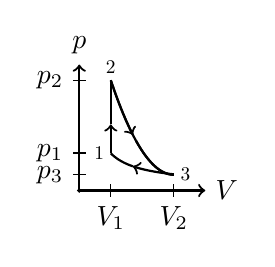
\begin{tikzpicture}[ scale=.4,baseline={(0,0)}]
%\draw (0,0) grid (4,4);
% x-axis
\draw [thick,->] (0,0) -- (4,0) node[right]{$V$};
% y-axis
\draw [thick,->] (0,0) -- (0,4) node[above] {$p$};
% x-axis label
%\node at (-0.3,4){$p$};
% y-axis label
%\node at (3.85,-0.4){$V$};
% origin point
\draw [color=black,fill=black] (0,0) circle (0.05);
%Isokor uppvärmning
\draw [thick,->](1,1.19) -- (1,2.1);
\draw [thick](1,2.1) -- (1,3.5)node[above,scale=0.7]{2};
%Isentropis expansion
\draw[ thick,domain=1:3, smooth, variable=\x, black] plot ({\x}, {(0.5+(3.5-0.5)*(abs((\x-3)/(1-3)))^2});
\draw[ thick,->,domain=1:1.7, smooth, variable=\x, black] plot ({\x}, {(0.5+(3.5-0.5)*(abs((\x-3)/(1-3)))^2});
\draw[ thick,domain=1.8:3, smooth, variable=\x, black] plot ({\x}, {(0.5+(3.5-0.5)*(abs((\x-3)/(1-3)))^2});
%Want to use the below instead
% \coordinate (A) at (1,3.5);
%\foreach \x in {1,...,3}{
%\coordinate (B) at (\x,{(0.5+(3.5-0.5)*(abs((\x-3)/(1-3)))^2});
%%\draw[thick, black] (A)--(B) ;
%\ifthenelse{\x = 2.5}{\draw[thick,->,smooth, black] (A)--(B) ;}{\draw[thick,smooth, black] (A)--(B) ;}
%\coordinate (A) at (B);
%}
%Isoterm kompression
\node[scale=0.7, right] at (3,0.5) {3};
\draw[ thick,->,domain=3:1.7, smooth, variable=\x, black] plot ({\x}, {1/\x + 0.18});
\draw[ thick,domain=1.7:1, smooth, variable=\x, black] plot ({\x}, {1/\x + 0.18}); 
\node[scale=0.7, left] at (1,1.19) {1};
%Små streck på p-axeln 
\draw  (0.2,1.19) -- (-0.2,1.19) node[left] {$p_1$};
%\node at (-1,1.19) {$p_1$};
\draw  (0.2,3.5)--(-0.2,3.5) node[left] {$p_2$};
\draw  (0.2,0.5)--(-0.2,0.5) node[left] {$p_3$};
%\node at (-1,3.5)  {$p_2$};
%Små streck på V-axeln
\draw (1,0.2) -- (1,-0.2) node[below]{$V_1$};
%\node at (1, -1) {$V_1$};
\draw (3,0.2) -- (3,-0.2) node[below]{$V_2$};;
%\node at (2.5,-1) {$V_2$};
\end{tikzpicture}
}
%      \caption{Mät2 }
\label{fig1}
%  
%%%%%%%%%%%%%%%%%%%%%%%%%%%T-s-diagram
\subfigure[$T\mhyphen s$ diagram]
{
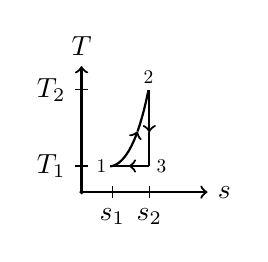
\begin{tikzpicture}[scale=.4,baseline={(0,0)}]
%\begin{tikzpicture}[show background rectangle, scale=.5]

%\draw (0,0) grid (4,4);
% x-axis
\draw [thick,->] (0,0) -- (4,0) node[right]{$s$};
% y-axis
\draw [thick,->] (0,0) -- (0,4) node[above]{$T$};
% x-axis label
%\node at (-0.3,4){$T$};
% y-axis label
%\node at (4,-0.3){$s$};
%origin point
\draw [color=black,fill=black] (0,0) circle (0.05);
%Isokor uppvärmning
\node[scale=0.7,left] at (1,0.83){1};
\draw[ ->,rotate=7,thick,domain=1:2, smooth, variable=\x, black] plot ({\x}, {(0.7 + (\x-1)^2});
\draw[ rotate=7,thick,domain=2:2.5, smooth, variable=\x, black] plot ({\x}, {(0.7 + (\x-1)^2}) node[scale=0.7,above]{2};
%Isentropis expansion
\draw [thick,->] (2.15,3.25) -- (2.15,1.9);
\draw [thick] (2.15,1.9) -- (2.15,0.83) node[scale=0.7,right]{3};
%Isoterm kompression
\draw [thick,->] (2.15,0.83) -- (1.5,0.83);
\draw [thick] (1.5,0.83) -- (0.98,0.83);
%Små streck på T-axeln 
\draw  (0.2,0.83) -- (-0.2,0.83) node[left] {$T_1$};
%\node at (-1,0.83) {$T_1$};
\draw (0.2,3.25) -- (-0.2,3.25) node[left] {$T_2$} ;
%\node at (-1,3.25)  {$T_2$};
%Små streck på s-axeln
\draw (0.98,0.2) -- (0.98,-0.2) node[below] {$s_1$};
%\node at (0,98, -1) {$s_1$};
\draw (2.15,0.2) -- (2.15,-0.2) node[below] {$s_2$};
%\node at (2.5,-1) {$s_2$};


%Pilar
%\usetikzlibrary {arrows.meta}
%\draw [arrows ={-Stealth[scale=1]}] (1.5,2.5) -- (1.5,1.9);
%\draw [arrows ={-Stealth[scale=1]}] (1.75,1.5) -- (1.75,1.0);
%\path (1.2,2.8) node  {$q_{till}$};
%\path (1.6,0.4) node  {$q_{\textit{bort}}$}; 

\end{tikzpicture}
}
%    \caption{Mät 2}
\label{fig2}
%\caption{Anpassning av $n$ i $p=\frac{C}{V^n}$}
\end{figure}

Den teoretiska termiska verkningsgraden $\eta_t$ definieras enligt
%\begin{wrapfigure}[5]{l}{0cm}
\begin{flalign*}
\eta_t &=\frac{q_{tillf}-|q_{bortf}|}{q_{tillf}} &\\
       &=1-\frac{|q_{bortf}|}{q_{tillf}} & (1) \\
\end{flalign*}
%\end{wrapfigure}
Avseende $q_{tillf}$ som ju är $q_{12}$ så rör vi oss till höger i $T\mhyphen s$ diagrammet.
Arean under kurvan blir således positiv därför att $ds>0$ om integrationsriktningen är positiv.\\
\begin{flalign*}
q_{12}&=\int_1^2 T\cdot ds &
\end{flalign*}
Värmemängdsändringen är således ändringen av den inre energin eftersom volymändringen är
noll i en isokorprocess $dv=0$
\begin{flalign*}
dq &= du + p\cdot dv &\\
dq &= \bar{c}_v\cdot dT + p\cdot 0 &\\
\end{flalign*}
Integration från 1 till 2 ger 
\begin{flalign*}
q_{12}&=\bar{c}_v\cdot(T_2-T_1) & (2)\\
\end{flalign*}
Problemställningen talar om en ideal gas men ger inget värde på $R$.

För en enatomig ideal gas gäller 
\begin{flalign*}
c_v&=\frac{3}{2}R &(3)\\
c_p&=\frac{5}{2}R &(4)\\
\end{flalign*}

För en tvåatomig ideal gas gäller 
\begin{flalign*}
c_v&=\frac{5}{2}R & (5)\\
c_p&=\frac{7}{2}R & (6) \\
\end{flalign*}
Vi antar helt godtyckligt att det rör sig om en enatomig ideal gas.
Förmodligen kommer gasspecifika faktorn att kunna förkortas bort då
kvoten $|q_{bortf}|/q_{tillf}$ beräknas.
 Således skriver vi
\begin{flalign*}
q_{tillf}&=\frac{3}{2}R\cdot(T_2-T_1) &\\
         &=\frac{3}{2}R\cdot(200-20)& (7)\\
\end{flalign*}
Värme bortförs under isotermen eftersom integrationsriktningen är omvänd, 
$q_{13}<0$, vilket också stämmer rent intuitivt. Om vi komprimerar gasen så stiger temperaturen men för att hålla
temperaturen konstant så måste vi hela tiden bortföra värmeenergi under komprimeringsprocessen.
Eftersom temperaturen på gasen inte ändras så ändras inte
inre energin $u_3-u_1=0$.
Ändringen av värmeenergin $q_{31}$ för isotermen från tillstånd 3 till 1 blir alltså lika med volymändringsarbetet $w_{31}$
$q_{31}=w_{31}$. 
\begin{flalign*}
q_{31}&= u_3-u_1 + w_{31} &\\
q_{31}&= 0 + w_{31} &\\
\end{flalign*}
Volymändringsarbetet för isotermen från 3 till 1 är per definition
\begin{flalign*}
w_{31}&=\int_3^1 p\cdot dv &\\
      &=\int_3^1\frac{R\cdot T}{v}dv &\\
      &=R\cdot T\cdot ln(\frac{v_1}{v_3}) &(8)\\
q_{bort}&=R\cdot T\cdot ln(\frac{v_1}{v_3}) &(9)\\
\end{flalign*}
Vi har dock ingen information om värden $p$ och $v$ sådant att vi kan räkna ut (9).
Vi ser dock att arean under kurvan i $T\mhyphen s$ diagrammet är en rektangel som vi
enkelt kan beräkna arean av såsom $(s_1 - s_3)\cdot T_1$.\\ 
Definitionen för entropi är
\begin{flalign*}
ds &= \bigg( \frac{dq}{T}\bigg)_{rev} &\\
   &=  \frac{du}{T} + \frac{p\cdot dv}{T} & (10)\\  
\end{flalign*}
för reversibla processer. Entropiändringen från 3 till 1
\begin{flalign*}
\int_3^1 ds &=\int_3^1 \frac{dQ}{T}&\\
s_1 -s_3 &= \int_3^1 \frac{1}{T}(du + p\cdot dv) & (11)\\
\end{flalign*}
För isotermen blir detta
\begin{flalign*}
 s_1 -s_3&= \int_3^1 \frac{1}{T}( 0 + p\cdot dv) &\\
         &=\int_3^1\frac{1}{T}\frac{R\cdot T}{v}dv &\\
         &=R\cdot ln(\frac{v_1}{v_3}) &\\
         &=R\cdot ln(\frac{v_1}{v_3}) & (12)\\
\end{flalign*}
Vi saknar information om $v_1$ och $v_3$ för att kunna använda denna.
Men $s_2=s_3$ så vi kan faktiskt räkna ut den sökta differensen
från isokor-processen därför att $s_2 -s_1$=$s_1 -s_3$
\begin{flalign*}
\int_1^2 ds &=\int_1^2 \frac{dQ}{T}&\\
s_2 -s_1 &= \int_1^2 \frac{1}{T} du + p\cdot dv &\\
         &= \int_1^2 \frac{1}{T} du + p\cdot 0 &\\
         &=\int_3^1\frac{1}{T}c_v\cdot dT &\\
         &=c_v\cdot ln(\frac{T_2}{T_1}) &\\
         &=\frac{3}{2}R\cdot ln(\frac{(273+200)}{273+20}) &\\
         &=\frac{3}{2}R\cdot 0.478922779&(13)\\
\end{flalign*}
Nu kan vi beräkna $(s_1 - s_3)\cdot T_1$ eftersom
$s_1 - s_3 =-(s_2 -s_1)=-\frac{3}{2}R\cdot 0.478922779$\\
Detta ger att
\begin{flalign*}
|q_{bort}|&=|(s_1 - s_3)\cdot T_1 &\\|
|q_{bort}|&=T_1\cdot \frac{3}{2}R\cdot 0.478922779 &(14)\\
\end{flalign*}
Vilket ger oss med insättning av (14) och (7)
\begin{flalign*}
\eta_t &=1-\frac{|q_{bortf}|}{q_{tillf}} &\\
       &=1-\frac{T_1\cdot \frac{3}{2}R\cdot 0.478922779}{\frac{3}{2}R\cdot(200-20)} &\\
       &=1 -\frac{(273+20)\cdot 0.478922779}{(200-20)} &\\
       &=1-0.779579858 = 0.220420142
\end{flalign*}
Korrekt svar måste anges med korrekt antal värdesiffror. Talet 200 har tre värdesiffror
och 20 har två värdesiffror. Talet 20 blir då bestämmande och svaret måste anges med
två värdesiffror. Således $\eta_t = 0.22$

%%%%%%%%%%%%%%%%%%%%%%%%%%%%%%%%%%%%%%%%%%%%%%%%%%%%%%%%%%%%%%%%%%%%%%%%%%%%%%%%%%%%
%%%%%%%%%%%%%%%%%%%%%%%%%%%%%%%%%%%%%%%%%%%%%%%%%%%%%%%%%%%%%%%%%%%%%%%%%%%%%%%%%%%%
%%%%%%%%%%%%%%%%%%%%%%%%%%%%%%%%%%%%%%%%%%%%%%%%%%%%%%%%%%%%%%%%%%%%%%%%%%%%%%%%%%%%
%%%%%%%%%%%%%%%%%%%%%%%%%%%%%%%%%%%%%%%%%%%%%%%%%%%%%%%%%%%%%%%%%%%%%%%%%%%%%%%%%%%%
%%%%%%%%%%%%%%%%%%%%%%%%%%%%%%%%%%%%%%%%%%%%%%%%%%%%%%%%%%%%%%%%%%%%%%%%%%%%%%%%%%%%
%%%%%%%%%%%%%%%%%%%%%%%%%%%%%%%%%%%%%%%%%%%%%%%%%%%%%%%%%%%%%%%%%%%%%%%%%%%%%%%%%%%%
%\end{multicols}
\end{document}
